\documentclass[12pt]{article}
\usepackage{hyperref}
\usepackage{natbib}
\usepackage{amsmath}
\usepackage{nicefrac}
\usepackage[usenames,dvipsnames]{xcolor}
\usepackage{graphicx}
\usepackage{footnote}
\usepackage{rotating}
%\usepackage{slashbox}
\usepackage{afterpage}
\usepackage{float}
\usepackage{color}

\usepackage[margin = 1.0 in]{geometry}
\usepackage{natbib}

\renewcommand{\bottomfraction}{.9}
\renewcommand{\topfraction}{.9}
\renewcommand{\textfraction}{0.1}
\renewcommand{\floatpagefraction}{.9}


%%%%%%%%%%%%%%%%%%%%%%%%%%%%%%%%%%%%%%%%%%%%%%%%%%%%%%%%%%%%%%%%%%%%%%%%%%%%
%   document style macros
%%%%%%%%%%%%%%%%%%%%%%%%%%%%%%%%%%%%%%%%%%%%%%%%%%%%%%%%%%%%%%%%%%%%%%%%%%%%
\def\gtrsim{\mathrel{\hbox{\rlap{\hbox{\lower4pt\hbox{$\sim$}}}\hbox{$>$}}}}
\def\lessim{\mathrel{\hbox{\rlap{\hbox{\lower4pt\hbox{$\sim$}}}\hbox{$<$}}}}
\newcommand{\ddg}{$\Delta\Delta G~$}
%%%%%%%%%%%%%%%%%%%%%%%%%%%%%%%%%%%%%%%%%%%%%%%%%%%%%%%%%%%%%%%%%%%%%%%%%%%%

\graphicspath{{../../analysis/figures/}}

\title{Sequence divergence as the main determinant of sequence-structure relationships}
\author{Amir Shahmoradi$^{1*}$, Eleisha L. Jackson$^2$, Claus O. Wilke$^2$}
\begin{document}

\date{\today}
\maketitle


\noindent
$^1$ Department of Physics, The University of Texas at Austin, Austin, TX 78712, USA \\
$^2$ Institute of Cellular and Molecular Biology, Center for Computational Biology and Bioinformatics, and Department of Integrative Biology, The University of Texas at Austin, Austin, Texas, 78712 USA\\

\bigskip
\noindent
$^*$Corresponding author\\
$\phantom{^*}$Email: amir@physics.utexas.edu\\
%$\phantom{^*}$Phone:{ \color{red} Need a phone} \\
$\phantom{^*}$Phone: +1 512 232 2459\\

\bigskip
\noindent
Manuscript type: research article\\
\bigskip
\noindent  Keywords: protein evolution, relative solvent accessibility, site variability


\begin{abstract}
Recent work has shown that structural properties are capable of predicting site-specific sequence variability for a given protein. However, the strength and significance of these structure-sequence relations appear to vary widely among different proteins, with absolute correlation strengths ranging from $0.1$ to $0.8$. Here we present the results from a comprehensive search for potential biophysical and structural determinants of protein evolution by studying more than $200$ structural and evolutionary properties in a dataset of $209$ monomeric enzymes. We discuss the main protein characteristics responsible for the general patterns of protein evolution, and identify sequence divergence as the main determinant of the strengths of virtually all structural-evolution relationships, explaining $10-30 \%$ of observed variation in sequence-structure relations. In addition to sequence divergence, we identify several protein structural properties that are moderately but significantly coupled with the strength of sequence-structure relations. In particular, proteins with more homogeneous back-bone hydrogen bond energies, large fractions of helical secondary structures and low fraction of beta sheets tend to have the strongest correlations between structural properties and site variability. 
\end{abstract}
\vfill
\vfill
\def\thefootnote{\fnsymbol{footnote}}
\setcounter{footnote}{0}


\section{Introduction}
\label{sec:intro}

{\color{blue}
The result in this paper: Site variabilty is the main determine of the difference in structure-sequence correlations. This is the main. It might be good to mention that we looked at 200 other predictors and found this as the more important one. The issue: There is a difference between the Huang et al paper vs. Sharamoradi et al. In Echave's paper with Huang or Yeh?, they say that the CN is the best predictor. In Amir's paper, we say that RSA is still the best predictor. Why is this different? The difference is in the datasets in terms of variability. This paper should have about 3 figures according to Claus possibly. So far I see 4 plots that need to be made: \\
1. WCN-Rate4site vs Mean RateSite??? Does this make sense? (Also for RSA) \\
2. WCN-Entropy vs Mean Entropy \\
3. RSA-Entropy vs Mean Entropy \\
Open Questions: Should I make the stress  and delta delta G correlations plots for the viral sequences that would complete the story?}


Proteins are subject to a number of biophysical and functional constraints \citep{Scherreretal2012, Wilkeetal2010}. These constraints result site-specific patterns of sequence variability within a protein. Recently several site-specific structural properties that can explain patterns of sequence variability in proteins have been identified. One of the earliest examples is Relative Site Accessibility \citep{Ramseyetal2011, Fransozaetal2009}. Residues that are buried in the core of proteins tend to be more conserved than exposed residues close to the surface of the protein.  Another structural property that has been found to significantly correlate with with site-specific variation is local packing density, often measured by Contact Number (CN) or Weighted Contact Number (WCN) \citep{Liaoetal2005, Yehetal2014, Huangetal2014}\\
\indent In a recent work, \cite{Echaveetal2015} presented a biophysical model that links the thermodynamic stability changes due to mutations at each site in proteins (\ddg)  to the rate at which mutations accumulate in the corresponding site over evolutionary time. They found that the variations in the free-energy of the protein due to amino acid substitutions at individual sites can explain the site-specific evolutionary rates comparable to the predictive powers of solvent accessibility and contact number. \\
\indent Although the majority of proteins exhibit some degree of correlation and association between sequence variation and structural properties, the strength of these correlations vary widely among different proteins. By analyzing a data set of $216$ monomeric enzymes, \cite{Yehetal2014} found a wide range of $\rho (\sim0.1-0.8)$ for the Spearman correlation strengths of sequence variability with two site-specific properties: the Weighted Contact Number (WCN) and RSA. Similarly, \cite{Echaveetal2015} recently found a wide range of $\rho\sim0.2-0.8$ for the correlation strength of the site-specific stability contribution -- quantified by \ddg -- with evolutionary rates. {\color{blue} It appears that sequence-structure correlations tend to correlate strongly with each other implying that several structural properties are representing similar biophysical constraints on site-specific evolutionary rates. SHOULD THIS BE IN RESULTS??} (Figure \ref{fig:seqent_structure_cors}). This implies that for a given protein, the correlation strength of a specific structural property with evolutionary rates can serve as a proxy for the correlation strength of other structural properties with sequence evolutionary rates. {\color{red} Where is the stress model, include it!!! Need to mention Huang Paper somewhere!}\\
\indent The fact that all relevant structural properties seem to have more or less the same predictive power for sequence variability implies the existence of one or more structural or evolutionary characteristics of proteins that modulate sequence-structure correlations in all proteins. The underlying principles behind the wide variation in correlation strengths among proteins in not well understood. Here we present the results of a comprehensive search for the potential underlying structural or evolutionary properties of proteins that can explain the wide range of variations seen in correlation strengths of sequence evolutionary rates with different structural properties.  We show that among all properties considered, {\color{blue}sequence divergence. What?? Can we discuss divergence when talking about entropy?} appears to be the primary determinant for the strength of sequence-structure relationships. In addition, we show that proteins with more homogeneous Hydrogen bond (H-bond) energies, higher fraction of Helical structures and lower number of $\beta$-sheets generally tend to exhibit the strongest sequence-structure correlations.  \\

\section{Materials and Methods}
\label{sec:mam}

    \subsection*{Structures, sequences, and measures of sequence properties } 
    The results presented in this work are based on a dataset of $209$ monomeric enzymes \citep{Echaveetal2015} randomly picked from the Catalytic Site Atlas $2.2.11$ \citep{Porteretal2004} with protein sizes in the sample ranging from $95$ to $1287$, including representatives from all six main EC functional classes \citep{Webb1992} and domains of all main SCOP structural classes \citep{Murzinetal1995}. To assess the evolutionary rates at the amino acid level for each protein, first a set of up to $300$ homologous sequences were collected by \citep{Yehetal2014, Huangetal2014} for each protein from the {\it Clean Uniprot} database following the ConSurf protocol \citep{Goldenbergetal2008}. Sequence alignments were then constructed using amino-acid sequences with MAFFT \citep{Katohetal2002, Katohetal2005}, specifying the auto flag to select the optimal algorithm for the given data set. The alignments were then used to calculate the site-specific evolutionary rates for each individual protein in dataset. To do so, we relied on two independent methods of measuring sequence variability measure. First, we calculated the Shannon entropy ($H_i$) -- the sequence entropy, hereafter abbreviated as {\it seqent} -- at each alignment column $i$:
    \begin{equation}
        \label{eqn:shannon}
        H_i = -\sum_j P_{ij}\ln P_{ij}
    \end{equation}

    where $P_{ij}$ is the relative frequency of amino acid $j$ at position $i$ in the alignment. The sequence entropy is a measure of variability at each site. We also calculated a measure of site-specific evolutionary rate -- hereafter abbreviated as {\it r4s} -- for each protein using software Rate4site {\color{red}(Citation??)}. First the Maximum Likelihood phylogenetic trees were inferred with RAxML, using the LG substitution matrix and the CAT model of rate heterogeneity \citep{Stamatakis2006, Stamatakis2014}. For each structure, we then used the respective sequence alignment and phylogenetic tree to infer site-specific substitution rates with Rate4Site, using the empirical Bayesian method and the amino-acid Jukes-Cantor mutational model (aaJC) \citep{Mayroseetal2004}.

    \subsection*{Calculation of Structural Properties}
    The goal of the presented work is to identify the prominent structural or sequence properties of proteins that modulate sequence-structure correlations. These potential modulators represent a unique characteristics of the protein as a whole.  In general, the structural and evolutionary properties fall into two major categories.  1. {\it Residue-level properties}: Site-specific structural or evolutionary properties that are defined and calculated for each specific amino acid site in the protein sequence. Prominent examples of the site-specific structural properties include RSA \citep{Fransozaetal2009, Scherreretal2012, Yehetal2014}  and WCN \citep{Shihetal2012, Yehetal2014} {\color{red}Should I cite Lin paper?}.   2. {\it PDB-level properties}: structural or evolutionary characteristics that are representative of the protein as a whole. Examples include protein Contact Order (CO) as defined by {\color{red}Need Citation!}, protein size and compactness, sequence length, and structural resolution of the protein in X-ray crystallography. {\color{blue} RE-WRITE THIS In addition, the distribution of each residue-level property can be summarized by its statistical moments as protein-level property of the protein}. Prime examples include, the mean and variance of WCN, RSA, sequence entropy, evolutionary rates. A comprehensive list of protein properties and their definitions are given in Table 
 \ref{tab:definitions} {\color{red} Where is this table???!!!}. \\
\indent A popular tool in condensed matter physics, Voronoi tessellation of a set of points (seeds) is a way of dividing the space into a number of regions such that for each seed there will be a corresponding region consisting of all points closer to that seed than to any other. These regions are called Voronoi cells. The structure of proteins can be considered as a set of 3D coordinates representing individual sites. We use VORO++ software {\color{red}(Need citation!)} to calculate the relevant Voronoi cell properties of all sites in all proteins, and use DSSP \citep{Kabschetal2005}  for the calculation of Accessible Surface Area (ASA) for each site. We normalized the ASA for each site by the theoretical maximum solvent accessibility values of \cite{Tienetal2013}  to obtain the Relative Solvent Accessibility (RSA) for all individual sites in all proteins. In addition to ASA values, we also extract from DSSP output, information about the secondary structure of proteins such as the total number of residues participating in different types of helices, parallel or anti-parallel beta sheets, or loops and turns. To complete the list of pdb-level structural properties, we also calculate the Spearman correlations between all residue-level structure and sequence properties and include them in the analysis to probe their potential effects on the strength of structure-sequence relations. \\

    \subsection*{Eliminating Degeneracy in Structural Property Definitions}
    In order to identify the potential determinants of sequence-structure correlations, we first ran a comprehensive search to identify site-specific structural properties that might correlate with measures of sequence variability (i.e., seqent \& r4s). There are however degeneracies in the definition of the some site-specific variables. For example, the quantity WCN is generally calculated from the coordinates of $\alpha$-carbon atoms in the 3-dimensional structure of proteins. There is however no reason to believe this set of atomic coordinates are the best representatives for individual sites in proteins. The same definition degeneracy also exists for the set of atomic Bfactors {\color{red}(Citation???)} that are used to represent site-specific flexibility, although the popular choice of residue flexibility is $\alpha$-carbon atomic Bfactor \citep{Halle2002}. Thus, for the sake of comprehensiveness and in order to identify the best definitions of structural properties such as WCN, Bfactor, and Voronoi cells, here we calculate and consider all possible definitions of properties depending on the choice of the representative set of atomic coordinates used. These include the set of coordinates of all backbone atoms ($N$, $C$, $C_\alpha$, $O$) and the first heavy atom in the amino acid side chains ($C_\beta$). In addition, we calculate representative coordinates for each site in protein by averaging over the coordinates of all heavy atoms in the side chains. We also calculate a representative coordinate for each site that is an average over all heavy atom coordinates in the side chain and backbone of the amino acid. In rare cases where the side chain atoms are not resolved in the PDB file or the amino acid lacks the heavy atom needed (e.g., $C_\beta$ for Glycine). The coordinate for that specific site is replaced with the coordinate of the corresponding $C_\alpha$ atom in the amino acid backbone. Similar to WCN and Bfactor, there is also ambiguity as to which set of residue atomic coordinates best represent individual sites in proteins for the calculation of Voronoi cells.\\


All data and analysis scripts required to reproduce the work are publicly available to view and download at \url{https://github.com/shahmoradi/cordiv}.


\section{Results}
\label{sec:results}

    \subsection*{Average Side Chain coordinates as the Best Representation of Protein 3D Structure}
	{\color{red} CONDENSE THIS WHOLE SECTION. THIS IS COVERED IN HIS PAPER.}
        As explained in previous section, there is a high level of redundancy in the initial set of collected protein properties. In particular, depending on the set of atomic coordinates used, there are $7$ different measures for some residue characteristics such as the residue Weighted Contact Number, Bfactor and Voronoi cell properties. This in turn results in a large set of secondary variables at pdb-level that basically measure the same protein characteristics, but with different strengths.  Therefore, in order to eliminate redundant variables from dataset, we first compare the predictive power of different measures of residue characteristics based on the set of atomic coordinates used.m For the WCN we find that among all possible set of coordinates, the average over coordinates of all heavy atoms of each individual side chain results in WCN values that show the best correlation with other structural and sequence properties, such as RSA, Voronoi cell properties, sequence entropy, and evolutionary rates. Specifically, WCN from average side chain coordinates (wcnSC) outperforms WCN based on $C_\alpha$ coordinates (wcnCA) in predicting RSA, \ddg entropy, sequence entropy and evolutionary rates (r4sJC) by a median Spearman correlation difference of $0.09$, $0.10$, $0.07$ \& $0.08$, respectively (Figure \ref{fig:best_wcn}).\\ 
\indent For the measure of local flexibility in proteins (Bfactor) we similarly find that among all $7$ representative measures of site Bfactors, the average of Bfactor values over all heavy atoms of each individual side chain (bfSC) results in the best correlations with other structural and sequence properties. Specifically, bfSC outperforms the commonly used $C_\alpha$ Bfactor (bfCA) in predicting RSA, \ddg entropy, sequence entropy and evolutionary rates by a median Spearman correlation difference of $0.11$, $0.12$, $0.08$ \& $0.09$, respectively (Figure \ref{fig:best_bf}). Similar to WCN and Bfactor, the Voronoi cell properties, most importantly the cell surface area, volume and the cell compactness also correlate best with other structure and sequence properties, only if the average side chain coordinates are used as the seeds of Voronoi cells (Figure \ref{fig:best_voronoi}). All observations clearly demonstrate that individual sites in proteins are best represented by the average properties of the side chains of amino acids in the corresponding sites. In particular, the strength of structure and sequence correlations decrease when moving from side chain to backbone atoms. An exception to this general pattern is the correlation of the hydrogen-bond energies of the sites, which correlate more strongly with site characteristics calculated based on the backbone atoms instead of side chain. Based on the observations described in the previous paragraphs, we keep only variables measured from average side chain properties and coordinates throughout the rest of the analysis and omit all other similar measures that show only weaker correlations with other site-specific characteristics. The exclusion of these alternative measures results in a significant reduction in the number of pdb-level variables to be further analysed, without compromising generality and comprehensiveness of the analysis.\\

    \subsection*{Sequence divergence as the main determinant of Sequence-Structure Relation}
	{\color{red}COLOR Delta Delta G dor viral proteins???}
        In order to identify the potential contributing factors to the strength of sequence--structure correlations, we first employ one of the simplest nonparametric yet powerful tests of statistical dependence, that is, we construct the Spearman correlation matrix of all pdb-level structure and sequence properties. The choice of Spearman versus the popular Pearson's correlation measure is made in order to minimize the effects of any nonlinear variable relationships on the strengths of the correlations.  The resulting correlation matrix reveals a myriad of pdb-level properties each having a small but nonzero contribution to the strength of the structure-sequence correlations.
        \\
	
        A hierarchical clustering of the correlation matrix reveals two main independent factors that have the strongest influence on the strengths of sequence-structure correlations: 1. The sequence {\color{red} divergence} as measured by the standard deviation of sequence entropy and evolutionary rates (denoted by {\it sd.seqent} \& {\it sd.r4sJC}) among all sites in each protein structure.   2. The homogeneity of the hydrogen bond strengths among the backbone atoms of each protein structure, as measured by the standard deviation of hydrogen bond energies (denoted by {\it sd.hbe}) among all protein sites.   A reduced-size of the Spearman correlation matrix for the most influential factors on the two strongest sequence--structure (seqent$/$r4s -- wcnSC$/$varea) relations is illustrated in Figure \ref{fig:mainmods}.
        \\

        For the other weaker sequence--structure relations, i.e. the correlations of seqent$/$r4s with RSA, \ddg entropy (ddgent), and Bfactor (bfSC) we find other pdb-level properties that also contribute to the correlation strengths, comparable to or even stronger than in sequence divergence and hydrogen bond homogeneity. In general, we observe that for the weaker the sequence-structure correlations, factors that determine the accuracy of the measured residue properties become more influential on the strength of the correlations. In particular, the X-ray crystallographic resolution of the structure and the definition of the \ddg entropy play dominant roles, with Spearman correlation coefficients of $\rho~0.3$, on the strengths of the corresponding sequence-structure relations.
        \\

        To ensure the accuracy of the results obtained from the Spearman correlation matrix of the pdb-level properties, we also use multivariate linear regression models, with individual sequence-structure correlations as the sole regressand of the regression models, and the set of pdb-level properties as the explanatory variables.  Since the number of explanatory variables is comparable to the number of observations (i.e., the number pdb structures in the dataset), we use regularized regression {\color{red}(reference to R package xx)} on the entire dataset, and also on the rank transformation of the dataset in order to minimize the effects of potential nonlinearities in data. Depending on value of the free parameter $\alpha$, this generalized regression model is a compromise between {\it ridge regression} -- which attempts to shrink the coefficients of correlated predictors towards each other -- and {\it lasso regression} -- which tends to pick one of the correlated predictors and discard the rest. In addition to regularized regression, we have also employed Principal Component Regression (PCR) on the original dataset and its rank transformation. Both regression methods, PCR \& regularized, point to similar set of pdb-level properties as the strongest determinants of sequence-structure correlations.



\section{Discussion}
\label{sec:dcr}

        Throughout this work, we have carried out a comprehensive analysis in search for the main determinants of the strength of sequence--structure correlations -- some of which are newly reported and discussed in this work. Examples of sequence--structure relations include the correlations of sequence entropy ({\it seqent}) and measures of evolutionary rates (such as {\it r4sJC} used in this work) with measures of residue Contact Number (e.g., {\it wcnSC}), Relative Solvent Accessibility (RSA), \ddg entropy ({\it ddgent}). In addition, we have derived new site-specific properties, based on Voronoi Tessellation of protein 3D structures, that are comparable to or better than several previously known structural properties in explaining site-specific sequence entropy or evolutionary rates (e.g., Figure \ref{fig:seqent_structure_cors}). Prime examples include Voronoi cell volume ({\it vvolume}), surface area ({\it varea}) and Voronoi cell sphericity defined as,

        \begin{equation}
        \label{eqn:sphericity}
        \Psi = \frac{\pi^{\frac{1}{3}}(6V)^{\frac{2}{3}}}{A}.
        \end{equation}

        in which $V$ \& $A$ represent {\it vvolume} \& {\it varea} respectively. We have also shown that site-specific structural properties -- such as Weighted Contact Number, Bfactor and Voronoi Cell properties -- that are calculated from the average coordinates of side chain atoms, have the best explanatory powers for the sequence variability measures such as {\it seqent} and {\it r4sJC}. Compared to the common choice of back bone {\it CA} atomic coordinates, site-specific properties averaged over side chain atoms can outperform in predicting sequence evolutionary rates by as much as $0.12$ in terms of Spearman correlation strength.

        In search for the determinants of the strength of sequence-structure relations, we compiled a set of more than $200$ protein properties for a dataset of $209$ monomeric enzymes. By employing several independent parametric and non-parametric statistics, such as Spearman rank test, regularized regression and Principal Regression methods, we identify sequence divergence as the dominant factor in the strength of sequence-structure correlations, capable of explaining $10-30\%$ of the observed correlation strengths alone, in both the original and rank-transformed data.


\section{Acknowledgements}
The authors acknowledge the Texas Advanced Computing Center (TACC) at The University of Texas at Austin for providing High-performance computing resources. ELJ is is funded by a National Science Graduate Research Fellowship, grant number DGE-1110007. COW is funded by {\color{red} Which grants??}.  AS is funded by {\color{red} Which grants??}.
....

%\clearpage
%\newpage

%\cleardoublepage

\bibliographystyle{peerj} %"style
\bibliography{ej_manuscript_bib} %expected file "my refs.bib"

\section*{Figures}
%    \begin{figure}[tbh]
%            \begin{center}
%            %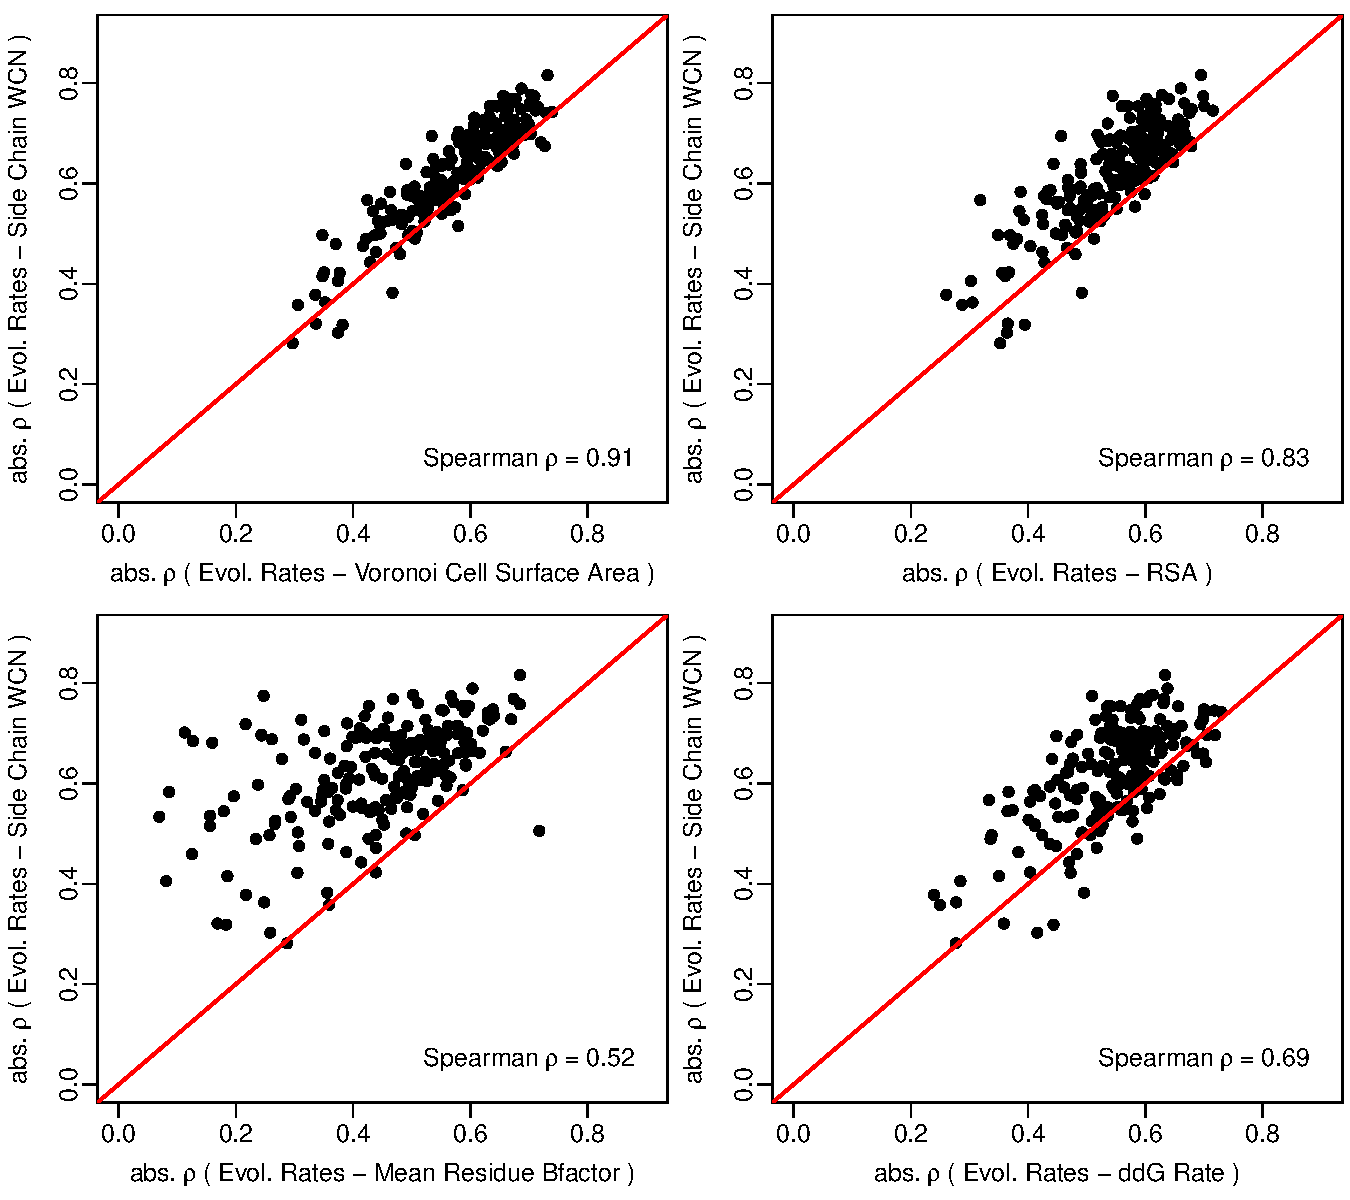
\includegraphics[width=6.9in]{cordiv_similarities_r4sJC.pdf}
%            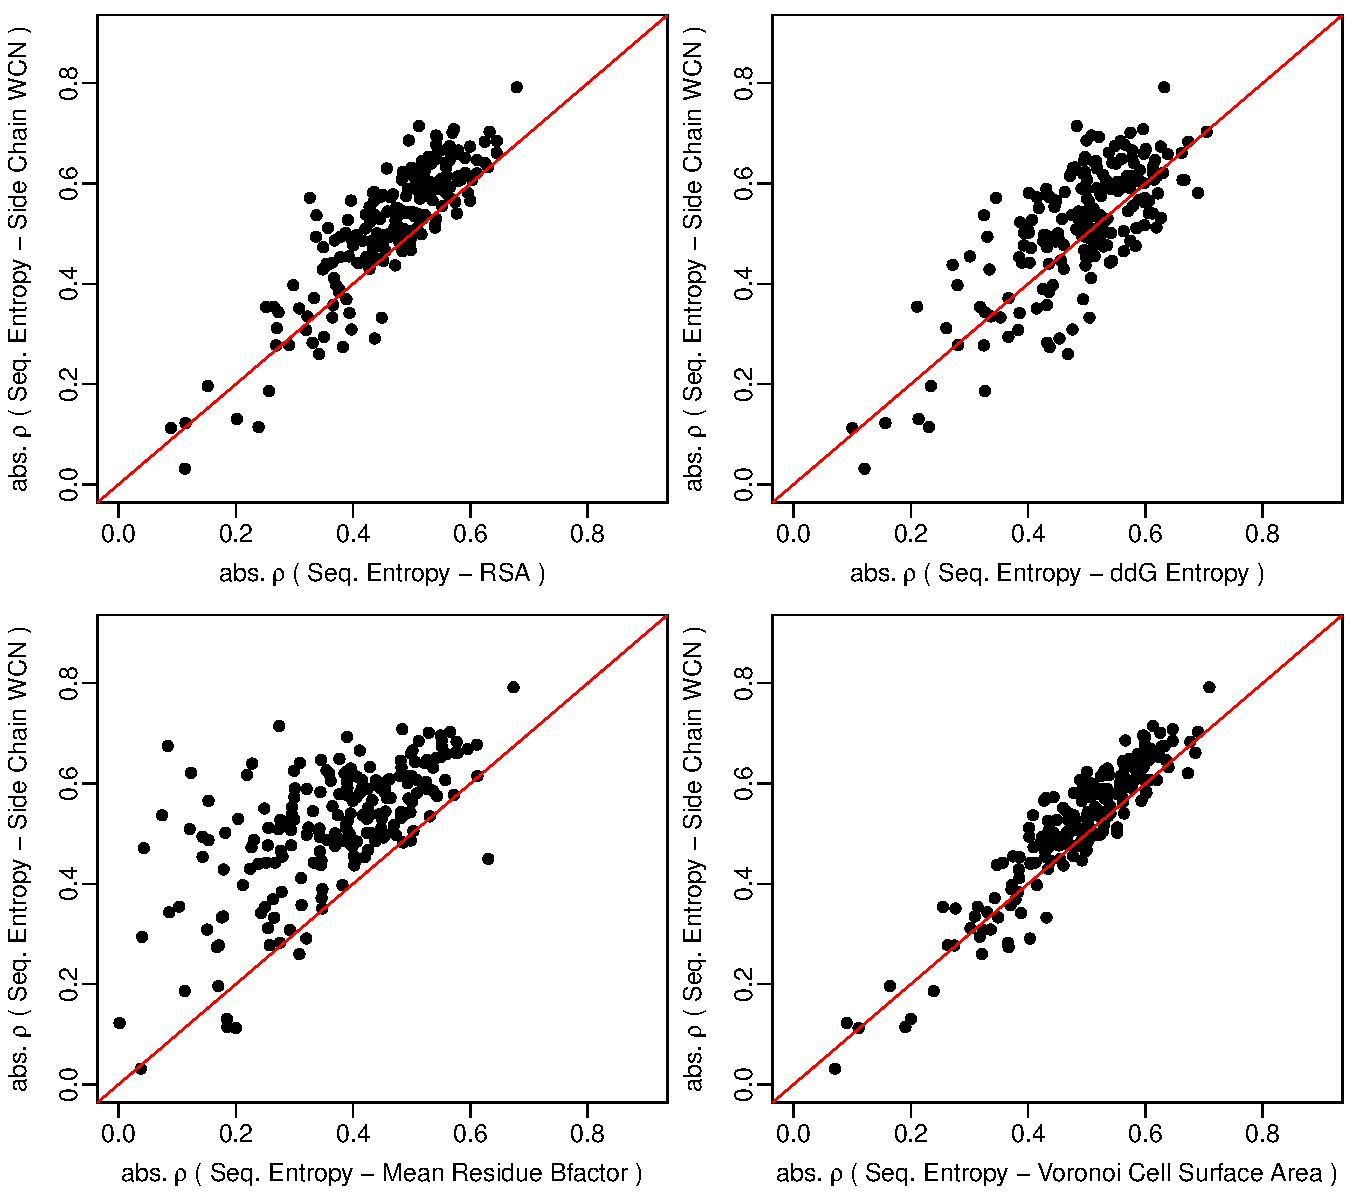
\includegraphics[width=6.9in]{cordiv_similarities_seqent.pdf}
%            \end{center}
%            \caption{A comparison of the strength of Spearman correlation of sequence evolutionary rates (r4sJC) with {\it side chain} Weighted Contact Number vs. correlations of other structural properties with evolutionary rates. Detailed description of the structural properties is given in Section \label{sec:mam}. The red lines in each plot represent equality line. It is evident from all plots that for any given protein in dataset, the correlation strength of one structural property is a good proxy measure of the correlation strength of any other structural property with sequence variability measures. For brevity, correlations of structure-rate4site are not shown here but are available online, also in supplementary material.}
%            \label{fig:seqent_structure_cors}
%    \end{figure}
%
%
%    \begin{figure}[tbh]
%        \centering
%        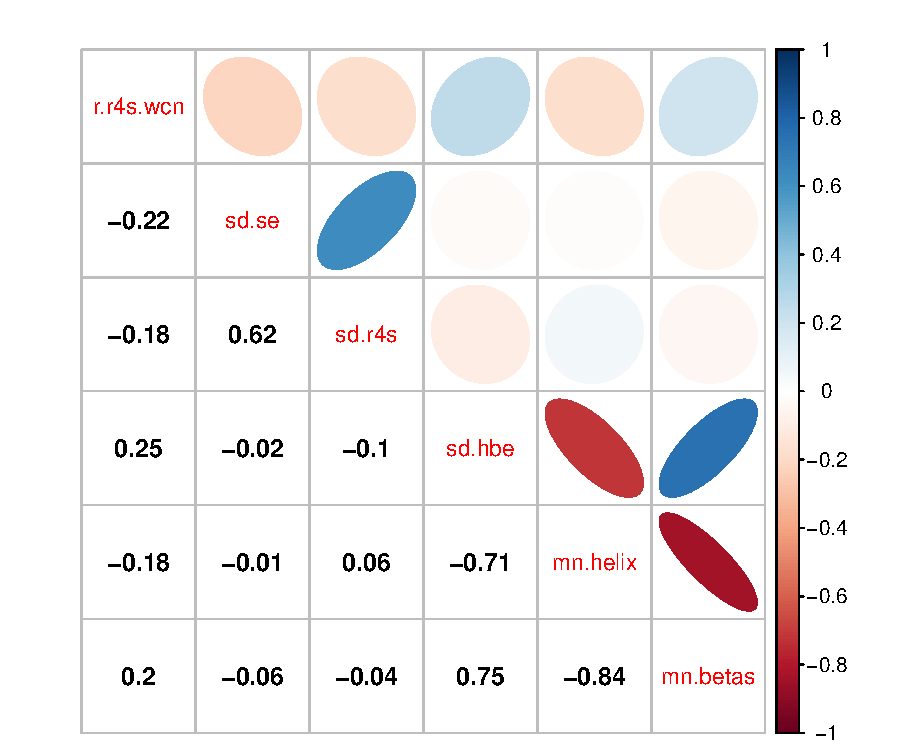
\includegraphics[width=3.6in]{/main_modulators_cormat_r4s_wcn.pdf} \\
%        \caption{{\bf The Spearman correlation matrix of the strongest sequence--structure correlations and the prominent determinants of the strengths of the corresponding relations}. The variables on the diagonal elements of the matrix from top to bottom represent respectively, the four strongest sequence--structure relations: r4sJC--wcnSC, r4sJC--varea, seqent--wcnSC, seqent--varea, followed by protein properties that modulate the strength of these relations: the correlation between r4sJC--seqent ({\it r.r4sJC.seqent}), variance of r4sJC ({\it var.r4sJC}), variance of sequence entropy ({\it var.seqent}), variance of back-bone hydrogen bond energies ({\it var.hbe}), and the fraction of amino acids in helical \& $\beta-$sheet secondary structures in the proteins ({\it mn.helix} \& {\it mn.betas} respectively).}
%        \label{fig:mainmods}
%    \end{figure}

%    \begin{figure*}[tbh]
  %      \centering
 %       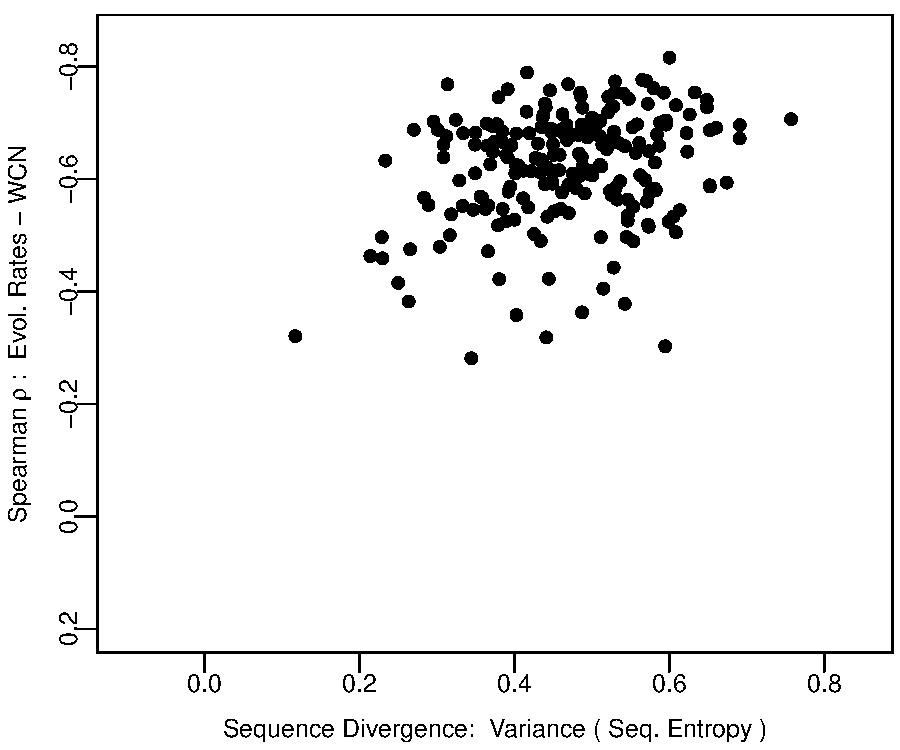
\includegraphics[width=3.4in]{/validation_r_r4s_wcn_var_seqent.pdf}
 %       \caption{{\bf Sequence--structure correlation strength versus sequence divergence.} The plot illustrates the relationship between the strength of a representative sequence--structure correlation ({\it seqent--scnSC}) and the sequence divergence as measured by the variance of protein sequence entropy. The black circles represent $209$ proteins used in this work. For comparison and validation, the red circles represent data for $9$ viral proteins taken from {\color{red}shahmoradi2014xx}}.
%        \label{fig:validation}
%    \end{figure*}

%    \begin{figure}[tbh]
%        \centering
%        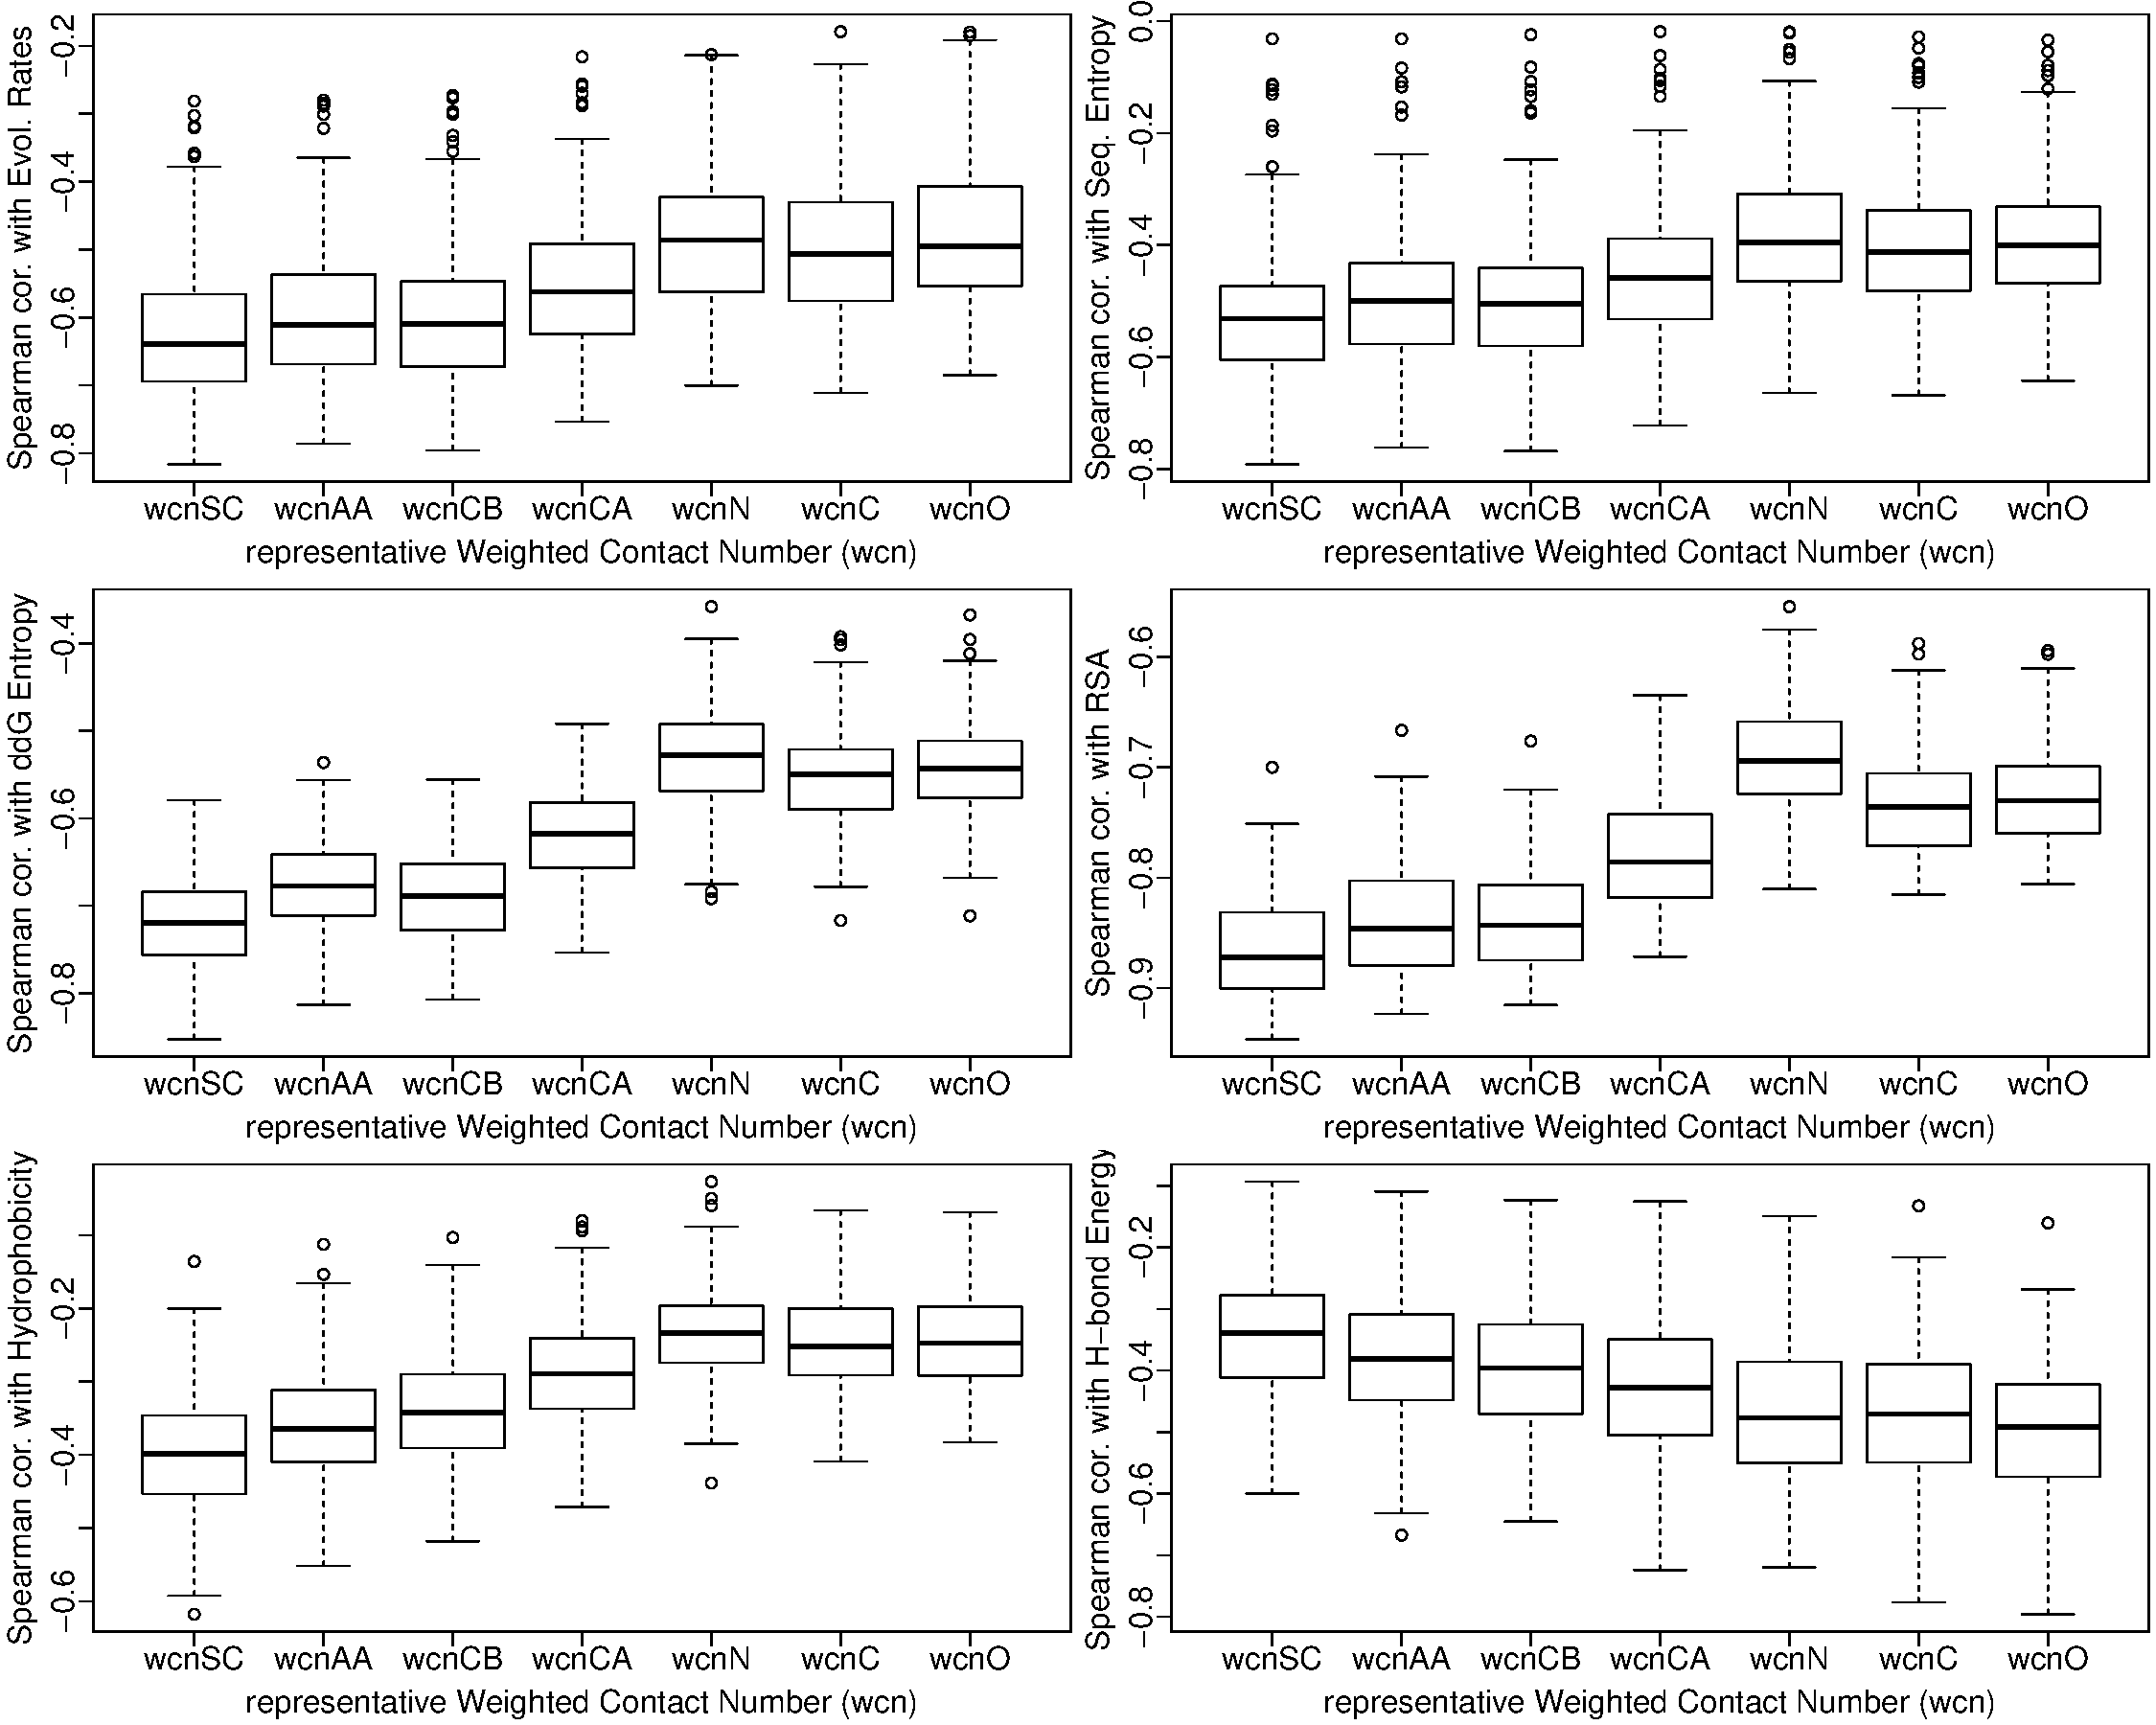
\includegraphics[width=7in]{/best_wcn/select_variables/boxplot_wcn_all_in_one.pdf} \\
%        \caption{NEEDS A CAPTION.}
%        \label{fig:best_wcn}
%    \end{figure}
%
%    \begin{figure*}[tbh]
%        \centering
%        \begin{tabular}{cc}
%        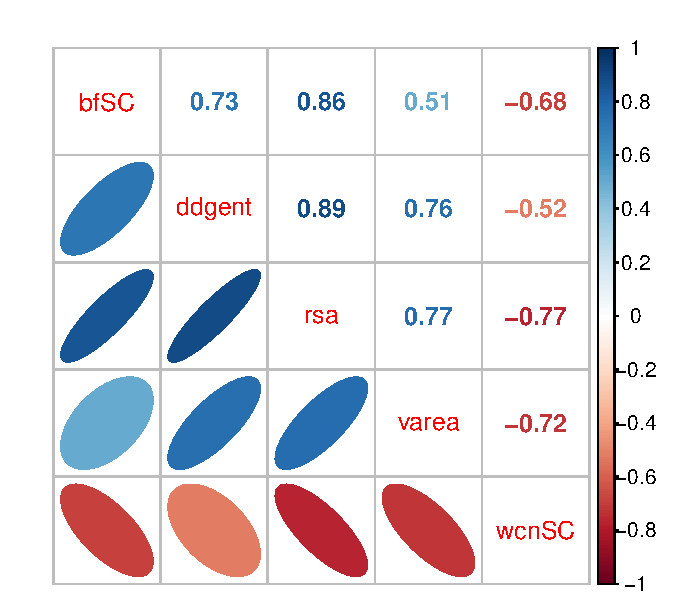
\includegraphics[width=3.4in]{/modulators_similarity_Sr4sJC_scors.pdf} & 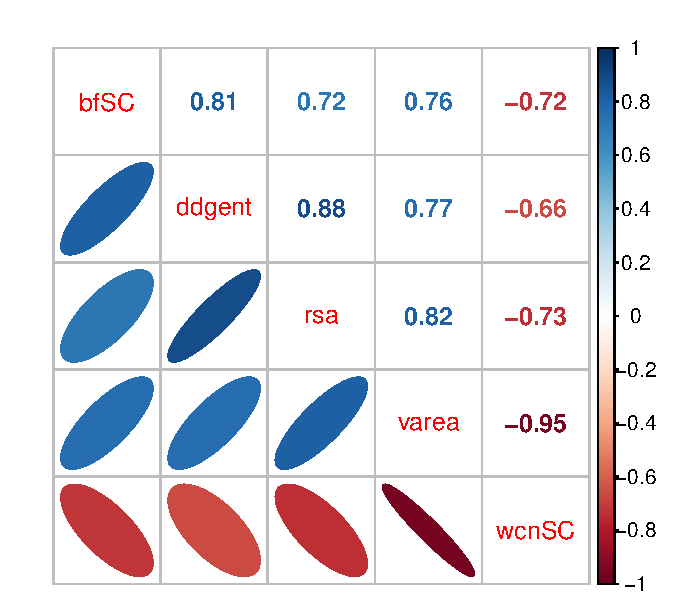
\includegraphics[width=3.4in]{/modulators_similarity_Sseqent_scors.pdf} \\
%        \end{tabular}
%        \caption{{\bf Spearman correlation matrices illustrating the similarity of the set of structure and sequence properties that contribute to the strength of sequence--structure relations}.  {\bf Left:} The correlation matrix for the relation of evolutionary rates ({\it r4sJC}) with structural quantities on the diagonal of the matrix. {\bf Right:} The correlation matrix for the relation of sequence entropy ({\it seqent}) with structural quantities on the diagonal of the matrix.}
%        \label{fig:simcormats}
%    \end{figure*}
%
    \begin{figure*}[tbh]
        \centering
        %\begin{tabular}{cc}
        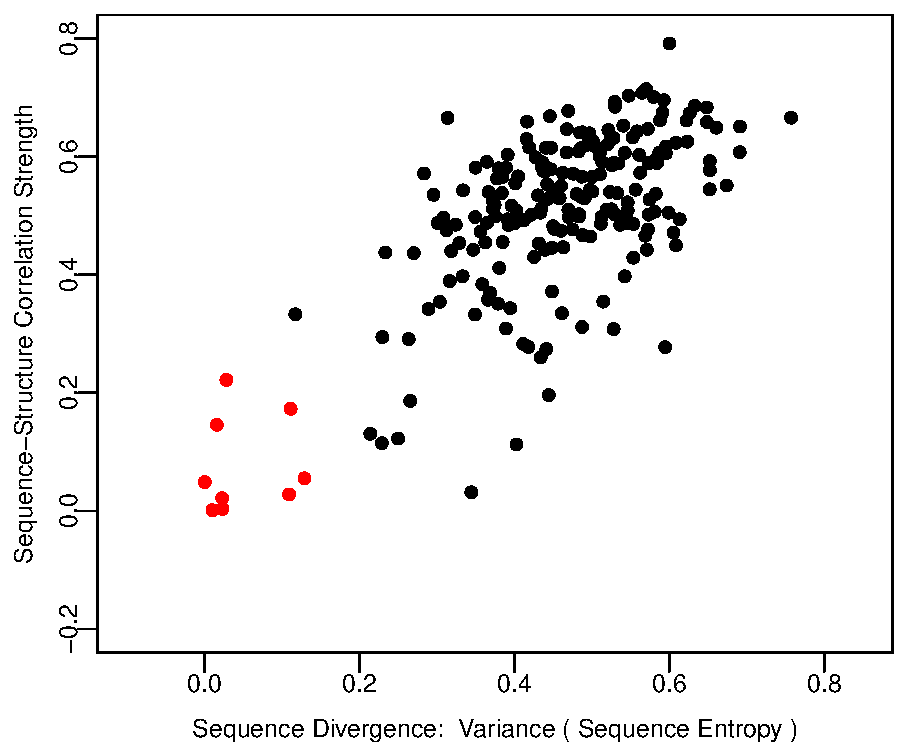
\includegraphics[width=3.4in]{/validation_r_seqent_wcn_var_seqent.pdf}
        %\end{tabular}
        \caption{{\bf Sequence--structure correlation strength versus sequence divergence.} The plot illustrates the relationship between the strength of a representative sequence--structure correlation ({\it seqent--scnSC}) and the sequence divergence as measured by the variance of protein sequence entropy. The black circles represent $209$ proteins used in this work. For comparison and validation, the red circles represent data for $9$ viral proteins taken from {\color{red} shahmoradi2014xx}}.
        \label{fig:validation}
    \end{figure*}

\end{document}

